\documentclass{article}
\usepackage[utf8]{inputenc}
\usepackage{amsmath,enumitem,wrapfig,pgfplots}
\usepackage{tikz,pgf-pie}

\usepackage{calc}

\usepackage[super,square]{natbib}
\usepackage{eso-pic}

\newlength{\PageFrameTopMargin}
\newlength{\PageFrameBottomMargin}
\newlength{\PageFrameLeftMargin}
\newlength{\PageFrameRightMargin}

\setlength{\PageFrameTopMargin}{1cm}
\setlength{\PageFrameBottomMargin}{1cm}
\setlength{\PageFrameLeftMargin}{1cm}
\setlength{\PageFrameRightMargin}{1cm}

\makeatletter

\newlength{\Page@FrameHeight}
\newlength{\Page@FrameWidth}

\AddToShipoutPicture{
  \thinlines
  \setlength{\Page@FrameHeight}{\paperheight-\PageFrameTopMargin-\PageFrameBottomMargin}
  \setlength{\Page@FrameWidth}{\paperwidth-\PageFrameLeftMargin-\PageFrameRightMargin}
  \put(\strip@pt\PageFrameLeftMargin,\strip@pt\PageFrameTopMargin){
    \framebox(\strip@pt\Page@FrameWidth, \strip@pt\Page@FrameHeight){}}}

\makeatother

\begin{document}

% Inspired by title template from ShareLaTeX Learn; Gubert Farnsworth & John Doe
% Edited by Jon Arnt Kårstad, NTNU IMT

\begin{center}
% Upper part of the page

\includegraphics[width=0.60\textwidth]{IISER-K_Logo.svg.png}\\[1cm]
\textsc{\LARGE IISER Kolkata}\\[1cm]
\textsc{\Large HU1102 - Sociology Dissertation}\\[0.5cm]
% Title

\centerline{\rule{1.2\linewidth}{.2pt}}
{ \huge \bfseries POLARIZATION IN SOCIETY: \\ A study on a selected group of population}\\
\centerline{\rule{1.2\linewidth}{.2pt}}


% Author
\Large
\emph{Authors:}\\
Abhratanu Ray - 22MS052\\
Aritra Barua - 22MS058\\
Debarshi Saha -22MS195\\
Niravra Nag - 22MS072\\
Sabarno Saha - 22MS037\\
\vfill
% Bottom of the page
{\Large Date : February 7, 2023}
\end{center}

\tableofcontents
\newpage
\section{Acknowledgement}
On behalf of our team, we would like to express our deepest gratitude to Dr. Sujata Sen for her guidance, support, and mentorship throughout the course of this dissertation. We are grateful for her willingness to make time for us, to answer our questions and to help us navigate the research process. We would also like to thank the IISER Kolkata for allowing us to use their valuable resources.
    \\ (two backslashes)
    \newline
    \hfill \break
We would also like to thank the University of Chicago Press, The Oxford University Press, The American Journal Of Political Science, The Annual Review of Political Science, The Elsevier Press and The American Behavioural Scientist Journal for publishing groundbreaking papers that have allowed us to understand the topic of our dissertation.
\\ (two backslashes)
    \newline
    \hfill \break
We are honored to have had the opportunity to work under Dr. Sen and we are confident that the knowledge and skills we have acquired during this study will serve us well in our future endeavors. Thank you, Dr. Sen, for your support, guidance and for being an excellent mentor.
\newpage
\section{Introduction}
Polarization in society refers to the growing divide between different groups of people, characterized by a lack of understanding and the inability to find common ground. It is a complex and multifaceted phenomenon that has been the subject of much research and discussion in recent years. This phenomenon can be observed in political, social, and cultural spheres, leading to increased tension and conflict among individuals and groups. 
In more recent times, this has become more and more visible to the common man, through means of social media and efficient communication facilities. We can now observe the polarization in our society, in real time. This makes it easier to spread radical ideas and hence create even more polarization. In our modern society, it has become an increasingly complex and interesting phenomenon.

This dissertation will attempt to study such a phenomenon, and decipher, at least to some small extent, its causes and effects. 

\newpage
\section{Methods Employed}
In this section, we lay down the methods we used to conduct our survey, data collection and study of the subject of polarization. We also describe the thought processes that led to us choosing the specific method we did.

\subsection{Previous Literature study}
For our study of polarization, we first delved into previous literature and studies conducted surrounding the topic of polarization in society, and other relevant areas, and then we studied 2 specific cases, in a way which highlighted the ways in which polarity was generated among people in these scenarios. The literature review is discussed on in Section 4. The case studies are also discussed under Section 5.1 and 5.2 respectively.
\subsection{Google Forms}
For our survey, we chose to design the questions in such a way that we would be able to make observations about how opinions differ across demographics, and how strongly people feel about polarization, and social conflict in our modern society.
The questions posed in the study are listed below.
\begin{enumerate}
    \item What is your age group?
    \item What is your level of education?
    \item What is your gender?
    \item Were you brought up in more of a traditional or modernized environment?
    \item Would you say you are closely associated with some political party/entity?
    \item If yes, please specify what party or entity. (This is optional)
    \item On a scale of 1 to 10, how likely are you to participate in vocal advocacy, for or against, some issue prevalent in society? 
    \item On a scale of 1 to 10, do you believe there needs to be an urgent and strong opposition to some current prevailing social trends?
    \item Have you previously been involved in some sort of vocal advocacy before, involving political or social issues (social media, rallies, etc.)?
    On a scale of 1 to 10, do you believe the views you develop on social or political issues are your own (as in examined and developed by you), or heavily influenced by opinions of family members, social media personalities or leaders?
    \item On a scale of 1 to 10, how likely are you to end associations or friendships over political differences, or disagreements on certain issues you hold close to you?
    \item On a scale of 1 to 10, do you believe your environment of upbringing has shaped a lot of the views you hold today?
    \item We also chose some case based questions.
    \begin{itemize}
        \item  Do you believe LGBTQ organizations are a positive force in society?
        \item Do you believe religious ideals are harmful to science and their coexistence is not possible?
    \end{itemize}

\end{enumerate}
We chose numeric scales for most questions as this allows us to analyze the data more efficiently, enabling us to statistically map the responses for people in different demographics, and revealing more information to us about the differences in opinions between people from different backgrounds, and how it leads to polarization among people in society. This results in a much more objectve and non biased survey since its done by a computer.
We perform this analysis later in this dissertation, (Section 5)

\newpage    
\section{Literature Review }
Polarization in today’s society is widely prevalent and of various types. It is on the rise throughout the world. Polarization in society refers to the growing divide between different groups of people, often characterized by their political beliefs, socioeconomic status, or other factors. This phenomenon has been the subject of much research and discussion in recent years, with scholars and experts from a variety of fields exploring its causes and effects.

One of the key drivers of polarization is the increasing political divide between left and right-leaning individuals and groups. Studies have shown that people are becoming more ideologically entrenched, with fewer people identifying as moderate and more identifying as either liberal or conservative. This has led to a growing divide in opinions and values between different groups, making it increasingly difficult for people with different beliefs to find common ground.
There are two distinct forms of political polarization. The first is ideological polarization, which is the divergence of political opinions, beliefs, attitudes, and stances of political adversaries\cite{Dalton1987-ps}.\\
The second is affective polarization, which is based on work considering the role of identity in politics .In contrast to ideological polarization, which mostly considers differences in political views, affective polarization is more of an identity-based comparison between in- and out-groups \cite{Iyengar2012-dw}. As such, it is defined as emotional attachment to in-group partisans and hostility towards out-group partisans (Hobolt et al., 2020). Thus, supporters of right-wing populist parties strongly oppose partisans of green or left-wing parties and vice versa, whereas both strongly favor their own fellow partisans. In large part affective polarization has increased over the last decades mostly due to an increase in out-party animus and not stronger affection for the own party \cite{Baldassarri2008-dn}\cite{Iyengar2019-ax}, as it has become widely acceptable to cast aspersions on supporters of other political parties.
 
Globalization played a role in decreasing polarization which was determined by researchers. ‘We found that the overall index of globalisation reduces polarisation. We found that economic and political globalisation negatively affect political polarisation. Furthermore, we used various robustness checks to verify that the suppressing effects of globalisation on polarisation are robust. Overall, we conclude that globalisation is beneficial to reducing polarisation ‘\cite{Fang2021-bh}
In modern times, especially since the growth of social media, polarization in society has taken a new turn and spreads more easily. Media is another channel to consider in determining polarisation. For instance, \cite{Bernhardt2008-wj}\cite{Melki2019-hl}, and Prior (2013)\cite{Prior2013-vz} show that media significantly affects polarisation. In general, greater freedom of the press decreases polarisation. Kubin and Sikorski (2021), recommend future research continues to explore ways media can be used as a tool to minimize polarization, rather than exacerbate it.
 
The Covid-19 pandemic also affected the social polarization and several works can be found on this. The COVID-19 pandemic poses a fundamental challenge for states and citizens around the world. Besides the drastic effects on economic systems and the well-being of individuals it also poses ramifications for the interaction between citizens and politics. So far there is suggestive evidence that the way parties and politicians handle the response to the corona crisis also influences the polarization of public opinion (van Bavel et al., 2020). If political debate is heavily split over the urgency of the crisis and how to handle it best, this can lead to greater polarization, too.
Despite the negative effects of polarization, some researchers argue that it can also have positive effects, such as increased political engagement and a greater diversity of opinions and ideas. LeBas, A. (2018)\cite{LeBas2018-hs}, argues that in certain cases where there exists a history of formal group exclusion or differential citizenship rights, political polarization is more likely to result in large-scale violence and democratic breakdown. Where power is strongly imbalanced, on the other hand, polarization is unlikely to be sustained, and the status quo ante will be retained. When these two conditions are absent, however, a relatively high degree of polarization can have surprising institution-building effects for new democracies. \\ \\ \\
\fbox{%
    \parbox{\textwidth}{%
    Overall, the literature suggests that polarization is a complex and multifaceted phenomenon that is driven by a variety of factors, including political ideology, social media, and economic inequality. While it can have negative effects on society, it can also have positive effects on political engagement and diversity of opinions.}%
}

\newpage
\section{Case Studies}
\subsection{Case Study 1: Farmers Protest}
\subsubsection{Background}
Despite the self- sufficiency of India in the production of food such as wheat, rice, fruits, vegetables and animal farming sectors, nutrition and hunger remain a serious problem in the country. According to the UN, India shares a quarter of the global hunger burden. \\
Studies have revealed that Indian farmers have small land holdings, even though part time farming is not a common practice. Thus, they are unable to meet their needs, which is one of the reasons contributing to the high rate of farmer suicides in the country. The slower growth of Punjab’s economy, particularly the agricultural sector, is believed to have fueled the protests.
\subsubsection{The Agriculture Laws}
There have been intentions of trying to increase the control of farmers over the sale of their produce, by encouraging direct trade with other buying parties outside the pre-existing APMC mandis, without the levying of any market fee. Former prime minister Manmohan Singh has expressed this desire in an interview in 2004, and it was quoted by current PM Modi in support of the reforms.

There have been international precedents in Kenya and the United States, where the agriculture policies were reformed to encourage private sector participation. While this increased the ease of doing business, there were many problems created for the small scale farmers, with their economic footholds based on the regulated prices being removed due to the privatization of the agricultural market.

The three acts that were passed in the parliament in September 2020 were as follows:
\begin{enumerate}
  \item Farmers' Produce Trade and Commerce (Promotion and Facilitation) Act: expands the scope of trade areas of farmers produce from select areas to "any place of production, collection, and aggregation. Prohibits state governments from levying any market fee, cess or levy on farmers, traders, and electronic trading platforms for a trade of farmers' produce conducted in an 'outside trade area'.
  \item Farmers (Empowerment and Protection) Agreement on Price Assurance and Farm Services Act: creates a framework for contract farming through an agreement between a farmer and a buyer before the production or rearing of any farm produces.
  \item Essential Commodities (Amendment) Act: allows for the center to regulate certain food items in the course of extraordinary situations like war or famine. Requires that imposition of any stock limit on agricultural produce be based on price rise.
\end{enumerate}
\subsubsection{Demands of The Farmers}
The immediate and the subsequent demands of the farmers were the repealing of the implemented Farm Laws, as they believed that opening the agricultural markets outside the APMC mandis will lead to detrimental effects on the finances of small scale farmers, as the stabilising effects of the Minimum Support Prices (MSPs) and the role of small scale agricultural businessmen, who provided support to farmers in the form of financial loans, timely procurement and assured regular prices, would be greatly diminished. The farmers were concerned that the market would be at the mercy of the corporates. 
\subsubsection{Factors and influences leading to the propagation of the social divide:}
As with any crisis that involves political entities and governments, the debates quickly diverged towards allegations that were unrelated to the direct cause of disagreement. We highlight a few such events.
\begin{enumerate}
    \item Several politicians have circulated misinformation and fake news about the protests, and based on this, have made allegations of separatism, sedition, and 'anti-national' activities concerning the farmers' protests. Many propaganda posts in support of the farm laws were made by various Indian Ministers, that were later revealed to either have been faked or earlier images that had been repurposed. The ruling party tried to destabilize the protests by associating “Khalistani” and similar separatist movements with the farmer protests, which were later verified to be false or exaggerated.\\
    \begin{center}
            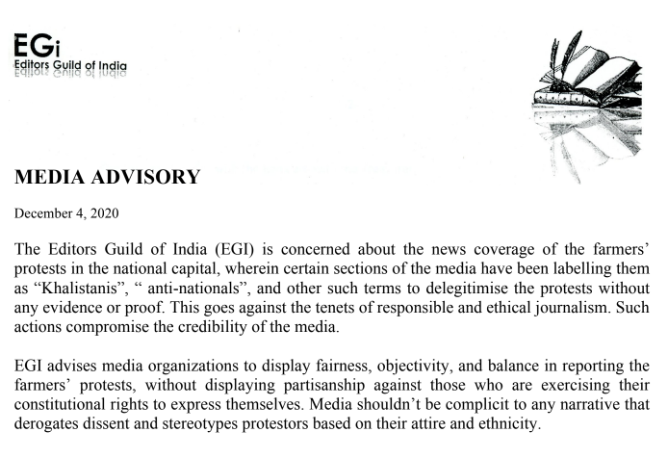
\includegraphics[width = 3 in]{pic1.png}
    \end{center}
    \item Many claims were also made that the protests had external conspirators that aimed to destabilize the Indian government and were being motivated by external forces like Chinese and Pakistani governments. There were also claims of ‘terrorists’ supporting and fueling the protests, as an attempt to swing nationalistic public opinion in favor of the government.
    \item Fake news tweets. Political capitalization of a sensitive issue, targeted provoking by political entities and certain media houses. We show an example of such a tweet by BJP IT cell head Amit Malviya. 
    \begin{center}
        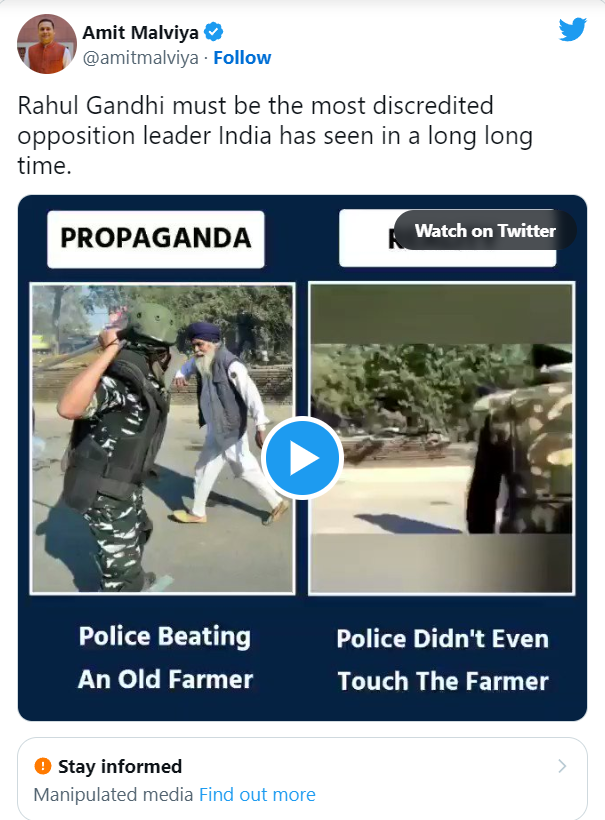
\includegraphics[width = 4.0 in]{pic2.png}
    \end{center}
    \item Former Chief Minister of Punjab, Parkash Singh Badal of the Shiromani Akali Dal returned his Padma Vibhushan award to the President of India on 3 December 2020, in his support of the farmers' protest. On 4 December 2020, environmentalist Baba Sewa Singh returned his Padma Shri Award. Punjabi folk singer Harbhajan Mann refused to accept the Shiromani Punjabi Award by the Punjab Languages Department of the Government of Punjab, India in support of the protests. Rajya Sabha MP and SAD(D) president Sukhdev Singh Dhindsa also announced that he would return his Padma award due to his personal support of the protests.
    \item There was major controversy regarding a tweet by young Swedish activist Greta Thunberg that contained a document outlining how to support the movement against the Indian Government, including the actions that one could take, hashtags which had the potential to trend on social media, and a list of celebrities who would be sympathetic to the cause of the protests. The government of India launched a probe and claimed that the toolkit was made by a Canadian pro-Khalistani organization based in Vancouver, that planned to carry out a campaign against the Indian government even after the protests ended, and if the laws were repealed. A Bangalore based activist, Disha Ravi was also arrested for allegedly creating and sharing the toolkit, with no further action being taken against her by the judgment of court.

    \item As fallout of the growing belief amongst protesting farmers that Mukesh Ambani and Gautam Adani were the principal beneficiaries of the farm laws enacted by the NDA Government, Punjab and Haryana farmers, in protest, decided to surrender Jio-sims and switch to rival networks. A number of Reliance Jio telecom towers and other infrastructure were damaged in Punjab in the last week of December 2020. Punjab Chief Minister Amarinder Singh appealed to the farmers to stop disrupting the communication towers.
\end{enumerate}
\subsubsection{Why were people motivated to become opinionated?}
There were various events, outlined below, which further caused people to choose one side over the other based on their personal point of view.
\begin{enumerate}
    \item After various incidents of violence at protests on 26th January 2021, the Republic Day of India, many farmers were forcibly removed from protest sites after problems faced by locals due to roadblocks, cuts in communication and various other supplies.
    \item On 26 January, tens of thousands of the farmers protesting agricultural reforms drove a convoy of tractors, earlier than the allotted time, to start the tractor rally into New Delhi. The farmers drove on prohibited routes in long lines of tractors, riding horses or marching on foot. However, a section of the tractor rally turned violent as the protesting farmers clashed with the police. Some of the protesters deviated from their pre-sanctioned routes permitted by Delhi Police and breached the barricades. Some protesters reached central Delhi and resorted to vandalism and damage to public property. Other protestors reached the Red Fort and hoisted the Nishan Sahib (a Sikh religious flag) and farmer union flags on the mast on the rampart of the Red Fort.
    \item On 27 September, farmer unions called a Bharat Bandh. The bandh had limited nation-wide impact. A protest on 3 October 2021 in Lakhimpur Kheri resulted in a number of deaths.
    \item On 20 December 2020, Facebook removed a page named Kisan Ekta Morcha, an official news source from farmers' protest. It was restored after public outrage. Since then both Facebook and Facebook-owned Instagram have been accused of removing and shadow banning content that spoke either in favor of farmers or against the BJP-led government, an accusation it has faced in the past too

\end{enumerate}
\subsubsection{A few personal observations and opinions.}
\begin{enumerate}
    \item The Central Government has used the Governors of the States as its puppets to block legislation of bills by the state governments of Punjab, Rajasthan and Chhattisgarh, which is a usual pattern of opposition to state governments using the Governors.
    \item The bills were repealed just before important elections in the states of Punjab and Uttar Pradesh, which was possibly a last minute move to win back the favor of some of the local people, another very common tactic.

\end{enumerate}



\newpage
\subsection{Case Study 2: CAA Protests}
\subsubsection{Background}
    On December 9, 2019, Home Minister Amit Shah submitted the Citizenship (Amendment) Bill, 2019 (CAB) on the floor of the Indian Parliament in reaction to the exclusion of 1.9 million persons, primarily Muslims and Hindus, from the National Register of Citizens for Assam. The Indian Parliament enacted the Citizenship (Amendment) Act, 2019 (CAA) on December 11. It modifies the Citizenship Act of 1955 to give a quicker route to Indian citizenship to anyone who entered India on or before December 31, 2014 and is a member of the designated minorities of Hindus, Sikhs, Buddhists, Jains, Parsis, and Christians from Afghanistan, Bangladesh, and Pakistan.\\ \\
The Act also aims to reduce the period of residency in India needed to obtain citizenship by naturalization for migrants covered by the Act from 11 to 5 years. The Act, however, makes no mention of Muslims and does not allow immigrants from those nations who practise other religions or Muslims the same eligibility privileges.\\ \\
The Act also makes no mention of any benefits for the other types of refugees that make up the majority of those residing in India, including the Rohingya refugees who were affected by the Rohingya genocide, the Sri Lankan Tamil refugees who were persecuted during the Sri Lankan Civil War, the Nepali refugees who were subjected to ethnic cleansing in Bhutan, and the Tibetan Buddhist
refugees who were persecuted in China.
\subsubsection{The Citizenship Laws}
THE CITIZENSHIP AMENDMENT ACT 2019 (An act to further amend the citizenship act 1955) In the Citizenship Act, 1955 (hereinafter referred to as the principal Act), in section 2, in sub-section (1), in clause (b), the following proviso shall be inserted, Provided that any person belonging to Hindu, Sikh, Buddhist, Jain, Parsi or Christian community from Afghanistan, Bangladesh or Pakistan, who entered into India on or before the 31st day of December, 2014 and who has been exempted by the Central Government by or under clause (c) of sub-section (2) of section 3 of the Passport (Entry into India) Act, 1920 or from the application of the provisions of the Foreigners Act, 1946 or any rule or order made thereunder, shall not be treated as illegal migrant for the purposes of this Act.
After section 6A of the principal Act, the following section 6B was added--
\begin{enumerate}
    \item The Central Government or an authority specified by it in this behalf may, subject to such conditions, restrictions and manner as may be prescribed, on an application made in this behalf, grant a certificate of registration or certificate of naturalization to a person
referred to in the provision to clause (b) of sub-section (1) of section 2.
    \item Subject to fulfilment of the conditions specified in section 5 or the qualifications for naturalization under the provisions of the
Third Schedule, a person granted the certificate of registration or certificate of naturalization under sub-section (1) shall be deemed
to be a citizen of India from the date of his entry into India.
referred to in the provision to clause (b) of sub-section (1) of section 2.
    \item On and from the date of commencement of the Citizenship (Amendment) Act, 2019, any proceeding pending against a person
under this section in respect of illegal migration or citizenship shall stand abated on conferment of citizenship to him: Provided that
such person shall not be disqualified for making application for citizenship under this section on the ground that the proceeding is
pending against him and the Central Government or authority specified by it in this behalf shall not reject his application on that
ground if he is otherwise found qualified for grant of citizenship under this section: Provided further that the person who makes the
application for citizenship under this section shall not be deprived of his rights and privileges to which he was entitled on the date of
receipt of his application on the ground of making such application.
    \item Nothing in this section shall apply to tribal area of Assam, Meghalaya, Mizoram or Tripura as included in the Sixth Schedule to
the Constitution and the area covered under "The Inner Line" notified under the Bengal Eastern Frontier Regulation, 1873.

\end{enumerate}
\subsubsection{Protests}
On December 4, 2019, after the bill was enacted, violent protests broke out across Assam, particularly in Guwahati and other parts of the state. Along with these major Indian cities, there were retaliatory demonstrations in Delhi, Bangalore, Ahmedabad, Hyderabad, Jaipur, Kolkata, and Mumbai.
At universities all over the nation, including Cotton University, Guwahati University, IIT Bombay, Madras University, Presidency
University, Kolkata, Jamia Millia Islamia, Osmania University, University of Hyderabad, University of Delhi, Punjab University, and Aligarh Muslim University, retaliatory demonstrations were also held. By the 16th of December, there were demonstrations in at least
17 cities across India, including Chennai, Jaipur, Bhopal, Lucknow, and Puducherry.
Between December 16 and December 18, 10,293 people from more than 1,100 universities, colleges, and academic institutions worldwide signed a declaration of support "condemning the recent police action and brutalization of students at Jamia Millia University and Aligarh Muslim University." The solidarity declaration was signed by academics from many of India's top universities, including JNU, Delhi University, all of the Indian Institutes of Technology, the Indian Statistical Institute, and the Tata Institute of Fundamental Research, among many others. Police detained professors and students from IIM-Ahmedabad on December 16 under the pretext that it was unlawful for them to demonstrate in opposition to the Act.
With the implementation of Section 144, which makes it illegal to congregate more than four people in a public place, authorities on December 19th prohibited protests in various areas of India, including parts of Bangalore, Uttar Pradesh, and the nation's capital, New Delhi. The IIM-Bangalore students participated in the Shoe Satyagraha, a peaceful protest against Section 144, by placing shoes and placards in front of the institute gate. IIM-Calcutta joined IIM-Ahmedabad and IIM-Bangalore in peacefully condemning the Act and the barbaric treatment of the students who were demonstrating across the nation by the police. From 19 to 22, several Kozhikodebased institutions, including IIM-Kozhikode, NIT-Calicut, Government Medical College, and Farook College, expressed their displeasure.
Chennai police refused to grant permission for any sort of manifestation, including marches and rallies. Additionally, internet access was cut off in some areas of Delhi. Numerous opposition politicians and activists, including Ramachandra Guha, Sitaram Yechury, Yogendra Yadav, Umar Khalid, Sandeep Dikshit, and D Raja, were detained as a result of the demonstrators' defiance of the prohibition. Tens of thousands of people demonstrated in Hyderabad, Patna, Chandigarh, Mumbai, and other cities despite their dread of being detained. Social media channels were used by political parties, civil society organizations, student groups, activists, and everyday people to urge participants to demonstrate peacefully. At Mumbai's August Kranti Maidan, 20,000 protesters peacefully
put an end to their demonstrations.

\subsubsection{The special case of the Northeast}
Assam received the majority of immigrants from 1951 to 1971, but other states did not, according to those who opposed the act. The CAA set 2014 as the cut-off date to define illegal foreigners. The new law would allow thousands of non-Muslim Bengali speakers from Bangladesh to immigrate legally to India, impacting the political and cultural landscape of Assam, which infuriated the protesters. On December 16, 17, and 18, thousands of All Assam Students Union (AASU) members and employees, as well as representatives from 30 other indigenous organizations, artists, and cultural activists from the state, assembled at Latasil Ground in Dispur to hold a satyagraha against the Act.
Access to the internet was restricted in Assam by the administrative authorities.[101] A curfew was also declared in Assam and Tripura due to the protests,[128] leading to army deployment as protesters defied the curfews. Railway services were suspended and
some airlines started to waive rescheduling or cancellation fees in those areas.

\subsubsection{Factors behind the Spurts in protests against CAA}
\begin{enumerate}
    \item First, one has seen a level of unprecedented polarization in society in the recent past. The debate today is rarely on issues and their relative merits and demerits. More often than not, the prism to decide the “stand" one takes on any socioeconomic or political development is where one “sits" in terms of the two ends of the political spectrum. So, if one supports the present ruling dispensation and its leadership, all its actions and decisions are seen as positive and in “national interest". Those opposing the initiatives are summarily dubbed as “anti-national". Those who seek to take decisions on the merits of every issue are unthinkingly dubbed as being
for or against the ruling establishment.  
    \item Second, compared to the decision to revoke Article 370 or the Supreme Court's ruling on the Ram temple-Babri Masjid controversy, the CAA and the Nation Register of Citizens (NRC) have sparked far more responses. Both the CAA and NRC influence a considerably larger portion of society. In the North-East, the issue has been examined from an insider-outsider perspective, but in majority of the country, the argument centres on whether religion should be the foundation of citizenship. The Bharatiya Janata Party (BJP) confronts
opposition in the North-East from both its allies and from factions inside the party.
    \item Third, while the citizenship bill was being debated in the two Houses, the Prime Minister was not present. It was left to the home minister to defend the stand of the government in both Houses. The equating of Partition with religion could well have been a tactical
error. The debate in the two Houses heightened tensions and could have well caused the unrest.
    \item Fourth, the involvement of the youth in the agitations got heightened after the developments in Jamia Millia University. Police action always invites a reaction.
    \item Finally, it's possible that not all of the protests you see on the street are organised or motivated by groups that oppose the coalition in power. The movement has been led by those who have been vehement opponents of the Congress and the Left, particularly in the North-East and in prestigious state-funded research institutes. By placing the responsibility for the demonstrations' intensity on a few specific political groups, one would be underestimating its magnitude. One can be underestimating the agitated social groups while
overestimating the power of such forces.
\end{enumerate}
\subsubsection{Impact of the Protests}
As the ongoing protest against the Citizenship Act turned violent, authorities of Guwahati University, Dibrugarh University and Cotton University postponed all semester exams scheduled up-to 16 December 2019. No play was possible on the fourth day of the cricket match between Assam and Services in the 2019–20 Ranji Trophy because of the protests. BCCI shifted two fixtures featuring three northeastern teams to other venues. The protests also affected the football matches of Northeast United, with their fixture against Chennai in getting postponed. The India-Japan summit in Guwahati, which was supposed to be attended by Japanese Prime Minister Shinzo Abe was also cancelled.\\ \\
The Indian Express reported that, during the second half of December, there had been a decline in the sales of cars, watches and other consumer goods, due to the ongoing protests.\\ \\
The demonstrations caused a number of trains, at least 700 flights, and more than 20 to be cancelled. After two railway stations in the state were set on fire, train service was entirely disrupted in certain areas of Assam. According to reports, the demonstrations caused property damage costs to the Indian Railways of 90 crore (US\$11 million), including losses of over 72 crore (US\$9.0 million) in West Bengal alone.\\ \\
Canada, France, Israel, Russia, Singapore, Taiwan, U.S. and the UK have issued travel advisories for nationals travelling to northeast India.\\ \\
The government imposed internet shutdowns in the states of Assam and Tripura, five districts in West Bengal, Bhopal, Dakshina Kannada and parts of Delhi. Mobile internet and SMS services were suspended in several places in Uttar Pradesh such as Lucknow,
Ghaziabad, Bareilly, Meerut and Prayagraj.

\section{Analysis}
\subsection{Data Tabulation}
For the google forms we got a total of 115 responses in total which are presented here in charts:
\begin{enumerate}
    \item What is your age group?\\ \\ \\
    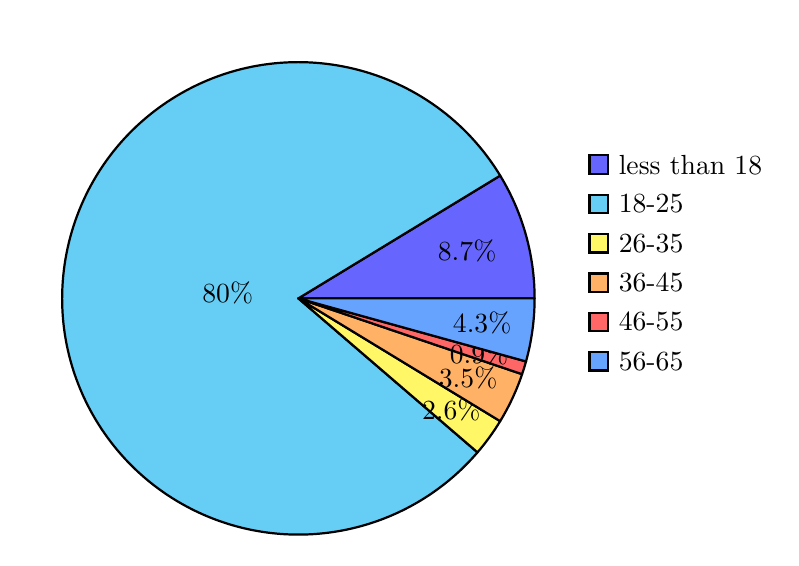
\begin{tikzpicture} 
    \pie[text=legend]{8.7/less than 18,80/18-25,2.6/26-35,3.5/36-45,0.9/46-55,4.3/56-65} 
    \end{tikzpicture}
    \newpage
    \item What is your level of education?\\ \\ \\
        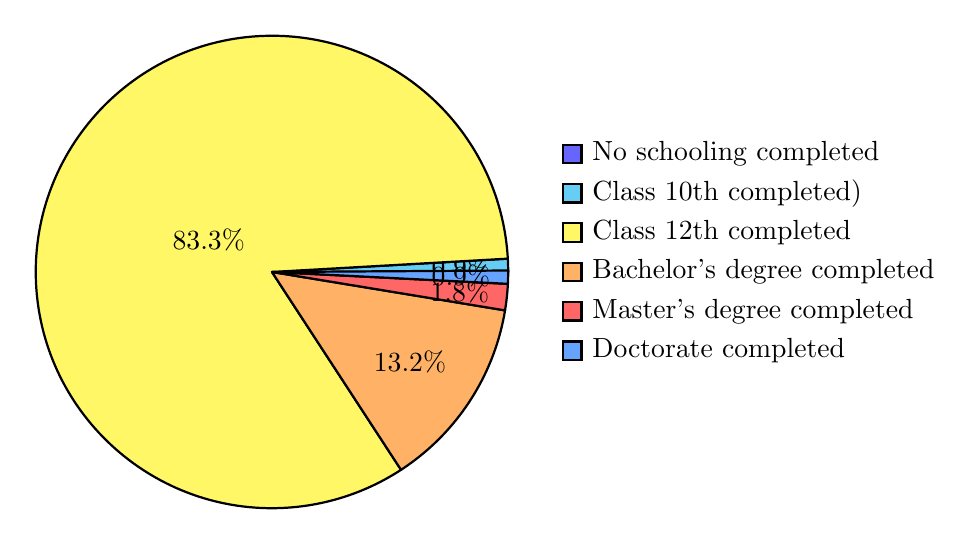
\begin{tikzpicture}
            \pie[text=legend]{0/No schooling completed,0.9/Class 10th completed),83.3/Class 12th completed,13.2/Bachelor's degree completed,1.8/Master's degree completed,0.9/Doctorate completed}
        \end{tikzpicture}
    \item What is your gender?\\ \\ \\
    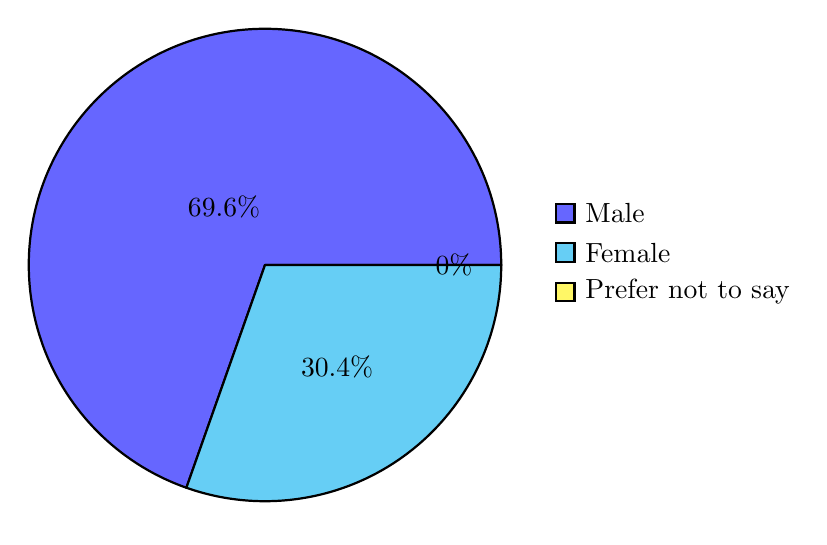
\begin{tikzpicture}
            \pie[text=legend]{69.6/Male,30.4/Female,0/Prefer not to say}
        \end{tikzpicture}
        \newpage
    \item Were you brought up in more of a traditional or modernized environment?\\ \\ \\
    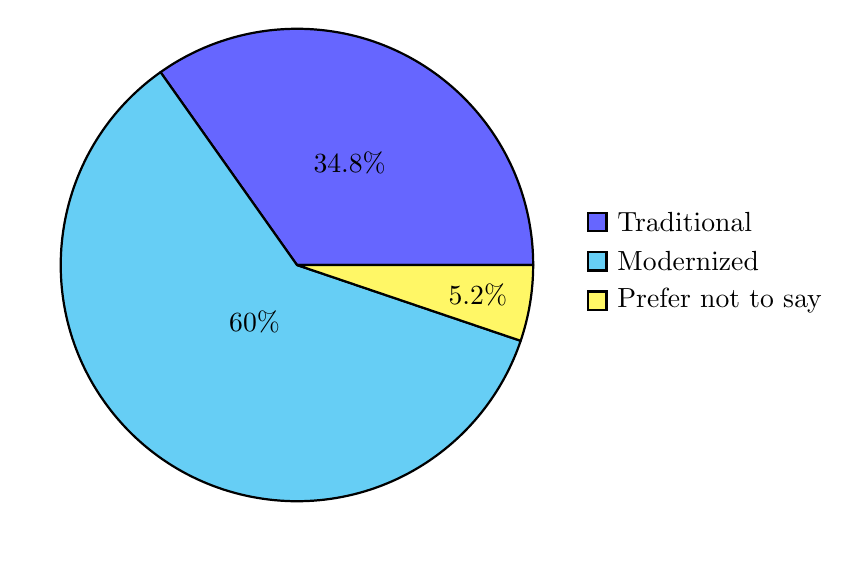
\begin{tikzpicture}
            \pie[text=legend]{34.8/Traditional,60/Modernized,5.2/Prefer not to say}
        \end{tikzpicture}
    \item Would you say you are closely associated with some political party/entity?\\ \\ \\
    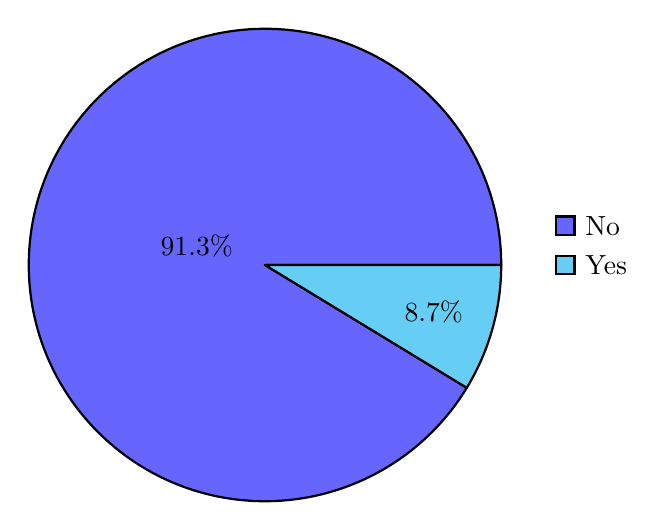
\begin{tikzpicture}
            \pie[text=legend]{91.3/No,8.7/Yes}
        \end{tikzpicture}
        \newpage
        \item On a scale of 1 to 10, how likely are you to participate in vocal advocacy, for or against, some issue prevalent in society? \\ \\ \\ 
    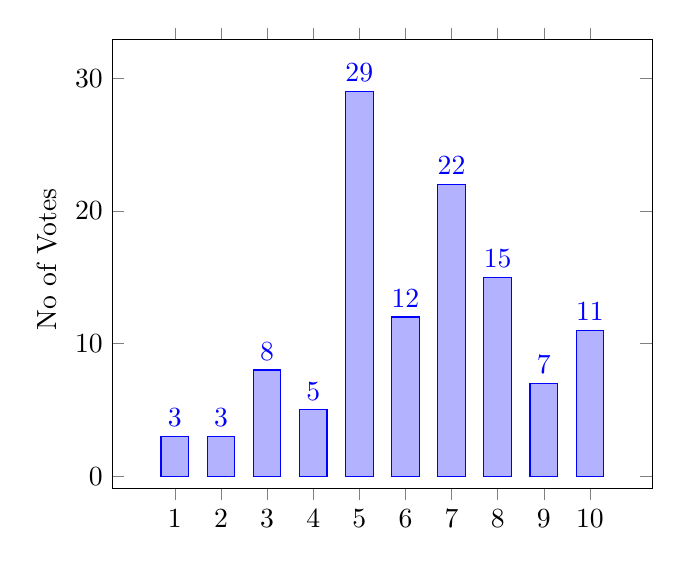
\begin{tikzpicture}
        \begin{axis}  
        [  
            ybar,  
            enlargelimits=0.15,  
            ylabel={\ No of Votes}, % the ylabel must precede a # symbol.
            symbolic x coords={1,2,3,4,5,6,7,8,9,10}, % these are the specification of coordinates on the x-axis.  
            xtick=data,  
             nodes near coords, % this command is used to mention the y-axis points on the top of the particular bar.  
            nodes near coords align={vertical},  
        ]  
    \addplot coordinates {(1,3) (2,3) (3,8) (4,5) (5,29) (6,12) (7,22) (8,15)(9,7)(10,11)};  
      
    \end{axis}  
    \end{tikzpicture}  \\ \\
    \parbox{\textwidth}{%
            “1” stands for “Not at all likely” and “10” stands for “Very likely”
            }% 
            \\ \\
    \item On a scale of 1 to 10, do you believe there needs to be an urgent and strong opposition to some current prevailing social trends?\\ \\
    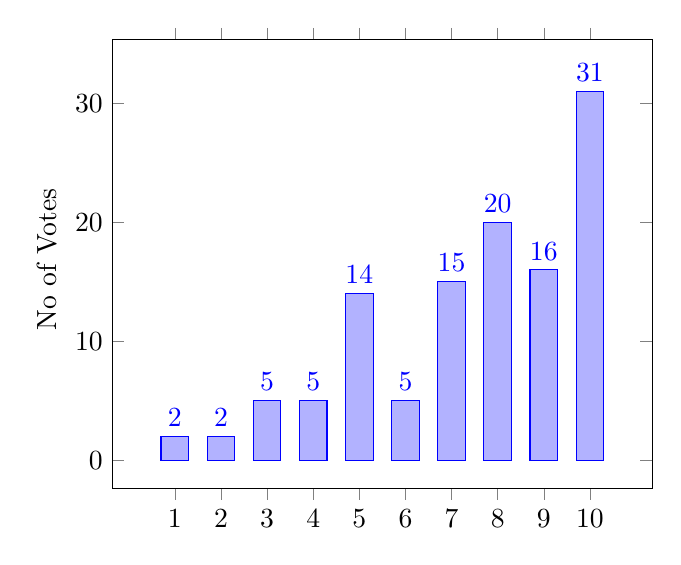
\begin{tikzpicture}
        \begin{axis}  
        [  
            ybar,  
            enlargelimits=0.15,  
            ylabel={\ No of Votes}, % the ylabel must precede a # symbol.
            symbolic x coords={1,2,3,4,5,6,7,8,9,10}, % these are the specification of coordinates on the x-axis.  
            xtick=data,  
             nodes near coords, % this command is used to mention the y-axis points on the top of the particular bar.  
            nodes near coords align={vertical},  
        ]  
    \addplot coordinates {(1,2) (2,2) (3,5) (4,5) (5,14) (6,5) (7,15) (8,20)(9,16)(10,31)};  
      
    \end{axis}  
    \end{tikzpicture}\\
     \parbox{\textwidth}{%
            “1” stands for “Not very urgent or necessary” and “10” Urgently necessary”            }%
            \\ \\
    \item Have you previously been involved in some sort of vocal advocacy before, involving political or social issues (social media, rallies, etc.)?\\ \\
    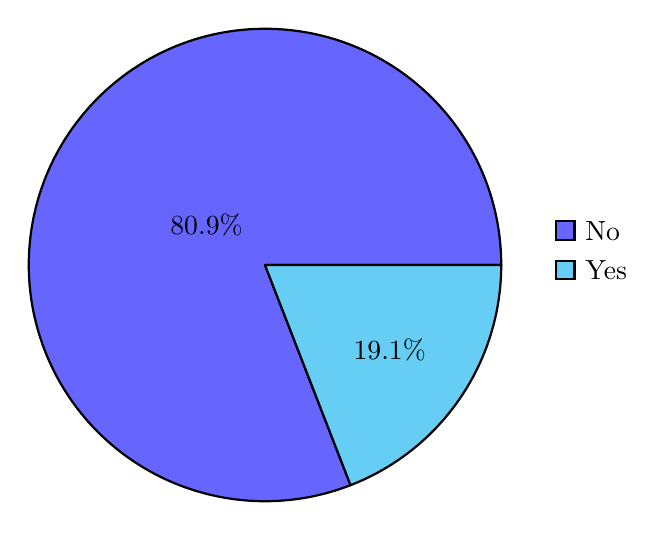
\begin{tikzpicture}
        \pie[text = legend]{80.9/No,19.1/Yes}
    \end{tikzpicture}
    
    \item On a scale of 1 to 10, do you believe the views you develop on social or political issues are your own (as in examined and developed by you), or heavily influenced by opinions of family members, social media personalities or leaders? \\ \\
    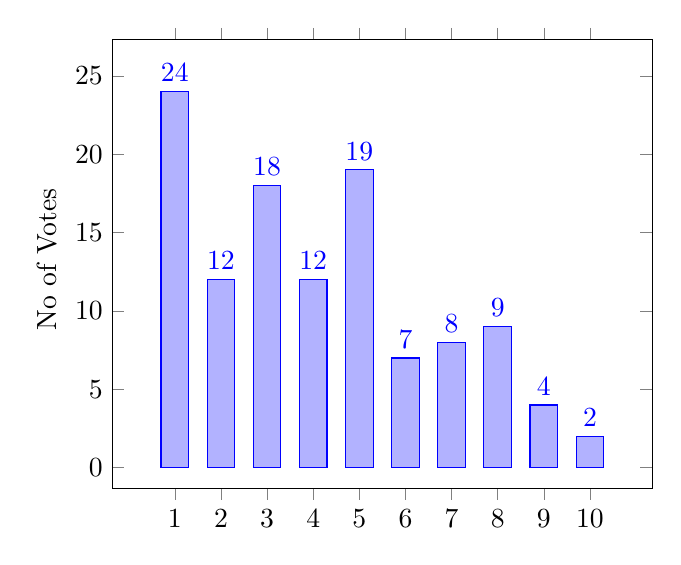
\begin{tikzpicture}
        \begin{axis}  
        [  
            ybar,  
            enlargelimits=0.15,  
            ylabel={\ No of Votes}, % the ylabel must precede a # symbol.
            symbolic x coords={1,2,3,4,5,6,7,8,9,10}, % these are the specification of coordinates on the x-axis.  
            xtick=data,  
             nodes near coords, % this command is used to mention the y-axis points on the top of the particular bar.  
            nodes near coords align={vertical},  
        ]  
    \addplot coordinates {(1,24) (2,12) (3,18) (4,12) (5,19) (6,7) (7,8) (8,9)(9,4)(10,2)};  
      
    \end{axis}  
    \end{tikzpicture}\\
     \parbox{\textwidth}{%
            “1” stands for “They are my own” and “10” stands for “Heavily influenced”
            }%
            \newpage
    \item On a scale of 1 to 10, how likely are you to end associations or friendships over political differences, or disagreements on certain issues you hold close to you?\\ \\
    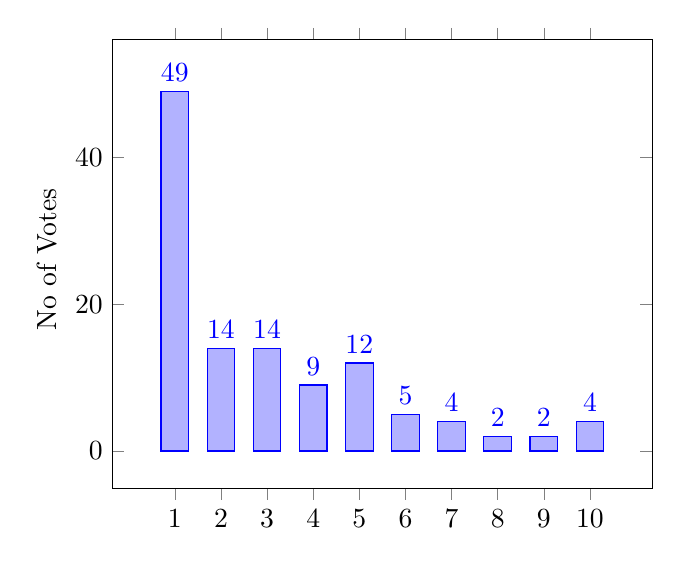
\begin{tikzpicture}
        \begin{axis}  
        [  
            ybar,  
            enlargelimits=0.15,  
            ylabel={\ No of Votes}, % the ylabel must precede a # symbol.
            symbolic x coords={1,2,3,4,5,6,7,8,9,10}, % these are the specification of coordinates on the x-axis.  
            xtick=data,  
             nodes near coords, % this command is used to mention the y-axis points on the top of the particular bar.  
            nodes near coords align={vertical},  
        ]  
    \addplot coordinates {(1,49) (2,14) (3,14) (4,9) (5,12) (6,5) (7,4) (8,2)(9,2)(10,4)};  
      
    \end{axis}  
    \end{tikzpicture}\\
     \parbox{\textwidth}{%
            “1” stands for “Not at all likely” and “10” stands for “Very likely”
            }%
    \item On a scale of 1 to 10, do you believe your environment of upbringing has shaped a lot of the views you hold today?\\ \\
    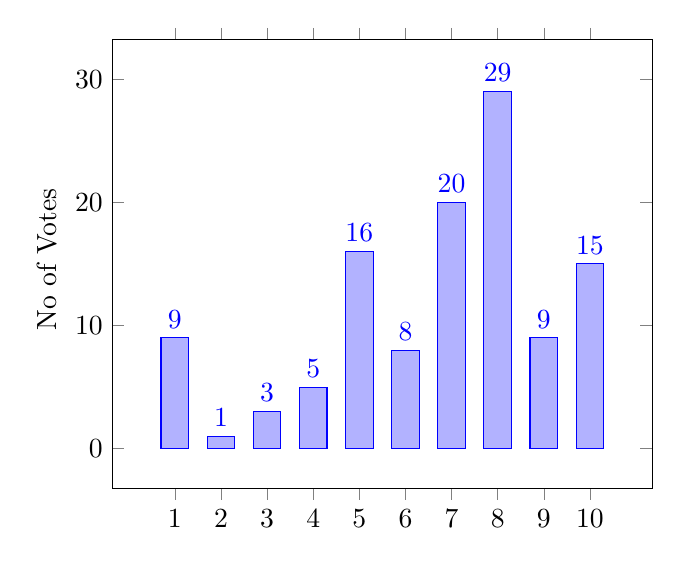
\begin{tikzpicture}
        \begin{axis}  
        [  
            ybar,  
            enlargelimits=0.15,  
            ylabel={\ No of Votes}, % the ylabel must precede a # symbol.
            symbolic x coords={1,2,3,4,5,6,7,8,9,10}, % these are the specification of coordinates on the x-axis.  
            xtick=data,  
             nodes near coords, % this command is used to mention the y-axis points on the top of the particular bar.  
            nodes near coords align={vertical},  
        ]  
    \addplot coordinates {(1,9) (2,1) (3,3) (4,5) (5,16) (6,8) (7,20) (8,29)(9,9)(10,15)};  
      
    \end{axis}  
    \end{tikzpicture}\\
     \parbox{\textwidth}{%
             “1” stands for “It hasn’t: and “10” stands for “It has”
            }%
    \newpage
    \item We also chose some case based questions.
    \begin{itemize}
        \item  Do you believe LGBTQ organizations are a positive force in society?\\ \\
        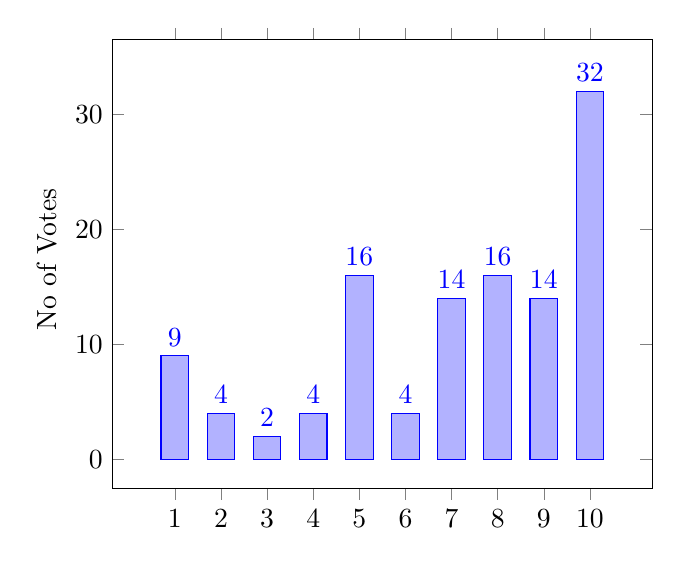
\begin{tikzpicture}
        \begin{axis}  
        [  
            ybar,  
            enlargelimits=0.15,  
            ylabel={\ No of Votes}, % the ylabel must precede a # symbol.
            symbolic x coords={1,2,3,4,5,6,7,8,9,10}, % these are the specification of coordinates on the x-axis.  
            xtick=data,  
             nodes near coords, % this command is used to mention the y-axis points on the top of the particular bar.  
            nodes near coords align={vertical},  
        ]  
    \addplot coordinates {(1,9) (2,4) (3,2) (4,4) (5,16) (6,4) (7,14) (8,16)(9,14)(10,32)};  
      
    \end{axis}  
    \end{tikzpicture}\\
     \parbox{\textwidth}{%
            “1” stands for “No, they are not” and “10” stands for “Yes, they are”
            }%
        \item Do you believe religious ideals are harmful to science and their coexistence is not possible?\\ \\
        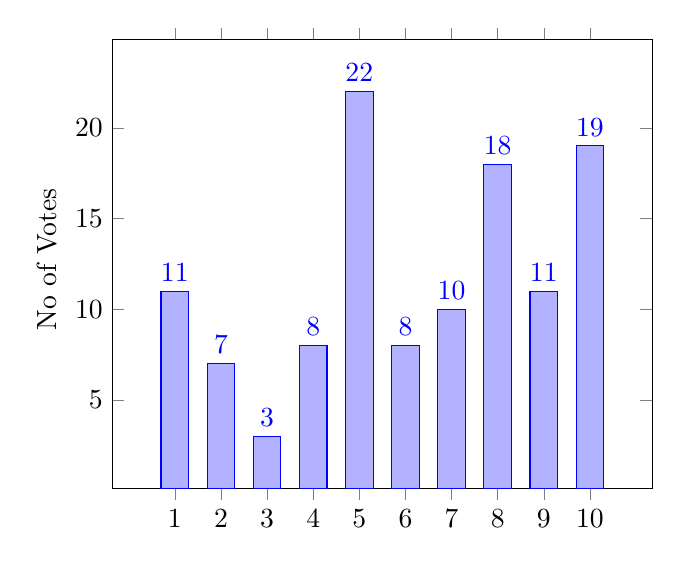
\begin{tikzpicture}
        \begin{axis}  
        [  
            ybar,  
            enlargelimits=0.15,  
            ylabel={\ No of Votes}, % the ylabel must precede a # symbol.
            symbolic x coords={1,2,3,4,5,6,7,8,9,10}, % these are the specification of coordinates on the x-axis.  
            xtick=data,  
             nodes near coords, % this command is used to mention the y-axis points on the top of the particular bar.  
            nodes near coords align={vertical},  
        ]  
    \addplot coordinates {(1,11) (2,7) (3,3) (4,8) (5,22) (6,8) (7,10) (8,18)(9,11)(10,19)};  
      
    \end{axis}  
    \end{tikzpicture}\\
     \parbox{\textwidth}{%
            “1” stands for “Yes, they are harmful” and “2” stands for “No, they aren’t harmful”
            }%
    \end{itemize}
\end{enumerate}
\newpage
\subsection{Statistical Analysis}
We observe that most people seem to agree with the questions presented in figures 2,3 and 4.
In general, we see the prevailing opinion to be that there exists a need for urgent change in certain aspects and trends of our society. People seem to feel strongly that there are some prevailing trends that are leading our society in unwanted directions. In figure 2, on a scale from 1-10, the average answer was 7.48, showing a deviation of 1.98 points towards the belief that there is a need for urgent change.
In figure 3, the respondents were asked whether or not they believe their opinions are influenced by some outside sources, perhaps by influencers or even their own family. The average response on a scale of 1-10 was seen to be 4.09, showing a deviation of 1.41 towards the belief that their opinions are not influenced by outside actors, but are rather their own. This shows that people believe their opinions are mostly their own, with little or no influence from their surroundings or the people around them.
In figure 4, respondents were asked how likely they are to end associations or friendships over political differences, or disagreements on certain issues they hold close to them. The responses to this question seem to be pretty unanimous, with an average response of 3.02, showing a deviation of 2.49 points towards them not being likely to end associations over disagreements on certain political/social issues. 
The fifth question, in figure 5, generated some more varied responses. The question posed was “On a scale of 1 to 10, do you believe your environment of upbringing has shaped a lot of the views you hold today?”. The average response came out to be 6.70, showing a deviation of 1.2 towards “It has.”, but the data set has a standard deviation of 2.5, showing that the data is accumulated in a wide range of values, that is, there is pretty large variation in the data, over the scale of 1-10. 
The two case based questions posed at the end of the survey show two very different results in the responses. For our first case based question, which was “Do you believe LGBTQ organizations are a positive force in society?”, there seems to be a very large range of opinions, with the standard deviation being 2.84. But, the mean came out to be 7.08, showing a pretty large deviation of about 1.58 towards “Yes, they are”, showing that most people tend to share a similar opinion, although the range of opinions is large, and there exist people on both ends of the spectrum. 
The second question we posed was “Do you believe religious ideals are harmful to science and their coexistence is not possible?”. This question had an even larger standard deviation of 2.85, but a mean value of 6.14, showing a small deviation of only 0.64 towards “No, they are not harmful”. This shows that there is no unanimous opinion among people, and there exist people on both ends of the spectrum. We can say this is a polarizing question, while the previous one is more of a uniting one. 

We now take a look at some demographic comparisons.
Comparing between genders, we find opinions of males and females to be pretty varied. 
Women are much more likely to participate in vocal advocacy for or against some political or social issue prevalent in society. The averages for men and women in the corresponding question (figure 1), are 5.91 and 6.97 respectively differing by over a whole point. 
Women also believe more strongly than men that there is a need for urgent social reform in our society. The averages for men and women in the corresponding question (figure 2) are 7.32 and 7.82 respectively, varying by 0.5.
In figure 3, the question posed was “On a scale of 1 to 10, do you believe the views you develop on social or political issues are your own (as in examined and developed by you), or heavily influenced by opinions of family members, social media personalities or leaders?”. The respective average responses for men and women were 3.93 and 4.45 respectively, showing a difference of 0.52. This shows that men believe themselves to be less influenced and more self educated or self inspired in their beliefs.
For figures 4 and 5, men and women seemed to agree reasonably well. But in figure 6, that is the first case based question, we see a very large difference in opinion. The average responses for men and women respectively were 6.43 and 8.57 respectively showing a variation of over 2 whole points. This indicates a very significant difference in opinion, showing women to be much more supportive of LGBTQ organizations. This indicates that gender, at least for this particular issue, seems to be a factor on which polarization has occurred, with women and men having different opinions.
For the second case based question, we also see a decent difference in opinion, with the difference being greater than 1 whole point. \\ \\
\fbox{%
    \parbox{\textwidth}{%
    Women and men tend to lean in the same direction, but women lean further in both cases. We hence see a difference in opinion, or rather a difference in the willingness to hold a strong opinion. Men seem to be more reluctant to state a strong opinion, with many men choosing more moderate options as compared to women. Women seem to show more assertiveness about their opinions, and are ready to be vocal about their beliefs as well.}%
}\\
\\
Next, we compare age groups.
Instead of comparing each age group separately, we decide to divide the respondents into 2 groups. The first group consists of all people under 18 and between 18-25 years of age. The second category contains people aged 26 and over, consisting of more middle aged people and senior citizens.
A surprising observation we obtain is that the older population is much more likely to participate in vocal advocacy than younger people (respective averages in figure 1 being 7 and 6.13). Also, older people seem to believe more strongly than young adults that there is a need for urgent change in society. Generally, throughout history it is the youth that are charged with an energy for change, and reform, while the older folks are more conservative; but this result portrays the contrary. This suggests that there is some factor in the socially normative culture of today, which polarizes the new and older generations.
For most other questions, both the opinions of older, and younger folks are in line with the general opinions, and are pretty similar. But we notice a very large difference when we get to the second case based question, that is, “Do you believe religious ideals are harmful to science and their coexistence is not possible?”. The averages for younger and older folks respectively, are 6.38 and 4.30, showing a pretty large difference in opinion. \\ \\\fbox{%
    \parbox{\textwidth}{%
    The younger folks seem to lean towards the belief that religious beliefs do not harm science, while older folks seem to believe they do. This is again a surprising result, since we expect the older population to be more conservative. }%
}

There are very large standard deviations in the for older age groups, indicating more varied opinions in older folks, and a wider range of opinions as well. Younger age groups have much smaller deviations, and more concentrated data.
We find that overall, younger and older groups seem to disagree on specific issues, more than their general outlook on society. Also, we surprisingly observe that the older population seems to be more socially active and vocally participative.

We now move on to comparing the demographics of the environment one grew up in, looking at whether someone grew up in a modernized or traditional environment.
People who grew up in a more traditional environment tend to believe their opinions are influenced by outside sources such as influencers, family members and relatives, much more strongly than people who grew up in a modernized environment. The averages for the traditional and modern categories are 4.77 and 3.65 respectively, showing people from modernized environments tend much more towards them believing their opinions to be wholly original than people from traditional environments do.
The opinions of people from modernized and traditional backgrounds showed quite a large variation when it came to the first case based question. The people from modernized backgrounds tend to be far more supportive towards LGBTQ organizations.  The averages for the modernized and traditional categories are 7.36 and 6.50 respectively, showing a pretty large difference of 0.84. \\ \\\fbox{%
    \parbox{\textwidth}{%
   This difference seems to be logical, given the fact that LGBTQ organizations have had a recent emergence in popular culture. It makes sense that people from modernized backgrounds are more accepting of them. So, in this case, the environment of upbringing and exposure one has, to new ideas, becomes a point of polarization in the batch.}%
}

Finally we will take a look at the opinions of people closely associated with political parties or organizations.
People closely associated with political organizations or parties, tend to be more vocally active and participative in political or social activism. Compared to the general population, the average responses to the first two questions by people associated with political parties ended up being much higher (7.5 and 8.7), that is, the two answers indicated that they strongly belief that there is an urgent need for change in today’s society and that the people associated with political parties are very willing to participate in activism as well. This makes sense, considering the fact that people associated with political parties generally tend to align their ideals with the more radical or opinionated aspects of the party they are a part of. They are also (in general) more educated about social dynamics and activism. 
\newpage
\section{Discussion and conclusion}
From our study, we have found some interesting observations and have managed to form an understanding of how polarization manifests itself within populations.
\newline
From section 4, we find that modern developments and advancements, especially in the areas of connectivity, globalization and political involvement (pointing at specific tactics like identity politics), have made it very easy for people to become polarized and agitated in very short periods of time. 
\newline
We see this confirmed through section 5, wherein subsections 5.1 and 5.2 highlight polarization occurring in real time, generated through the involvement of misinformation, provocative messaging and identity politics. We especially see this last element highlighted, where demographic differences are manipulated starkly by organisations, to romanticize certain events and play with people’s sentiments. Through targeted misinformation, labelling of people as extremists or “anti-nationals” for having differing opinions and various provocative social media campaigns, people have been swayed to ends of the spectrum and this manifests as radical ideas becoming more and more prevalent in our society.
\newline
The survey we conducted did mirror this in some ways, but seemed to show a lot more unity between demographics. Today, a lot of people seem to be tolerant of other’s ideals (section 6, subsection 6.1, point 10) and seem to agree on a few social issues, while they are still divided on others (section 6, subsection 6.2).
\newline
Still, people involved in political organisations seem to be the most opinionated, their opinions being more radical and differing from the rest of society by a decent margin. We also found older demographics to be more willing to participate, showing a growing disinterest among the youth towards activism and politics. Another interesting trend is that of women being more assertive, opinionated and ready to participate than men. 
These trends show changes in our society, differing vastly from the opinions and trends that were visible in our society just a couple decades ago. 
\newline
We end this dissertation by noting that although it is true that becoming polarized is easier and much more frequent today than it was in the past, we can still be hopeful, for we see most people from the generations of today seem to be ready to work together and understand differences in order to work out our problems.
\newpage

\bibliographystyle{plain} % We choose the "plain" reference style
\bibliography{refs} % Entries are in the refs.bib file

\end{document}
